% First we set up the style for the dissertation. Do not change this!
\documentclass[a4paper,oneside,11pt]{report}

% Now we load the preamble, which sets up most we need for the dissertation.
\usepackage[left=3.5cm,right=3.5cm,top=3cm,bottom=3cm]{geometry}
\linespread{1.25}

% Next we load some more packages. You might want to add to this list, but
% do not remove or change things unless you know what you are doing.

\usepackage{fancyhdr}
\pagestyle{fancy}
\rhead{Page~\thepage} % Page number at the top right.
\cfoot{} % No page number at the bottom.
\usepackage{graphics}
\usepackage{amsmath,amsfonts,amssymb,amsthm}
\usepackage{epsfig,epstopdf,color}
\usepackage{enumitem}
\usepackage[nottoc]{tocbibind}

% Note that we set some options for algorithm2e here. If you want another
% look to the result, change these.
\usepackage[english,algoruled,lined]{algorithm2e}

\usepackage{tikz}
\usetikzlibrary{arrows,automata}

% \usepackage[notcite,notref]{showkeys}
% Un-comment the line above this to see keys in the compiled output.

% Here is the place to put any more packages you need.

% The hyperref package is special: it has to be last.
\usepackage[hidelinks,breaklinks]{hyperref}

% Now we define a lot of commands and environments. The next five lines are
% options for enumerate.
\newcommand{\itm}[1]{\textrm{({#1})}} 
\newcommand{\itmit}[1]{\itm{\textit{#1\,}}} 
\newcommand{\rom}{\itmit{\roman{*}}} 
\newcommand{\abc}{\itmit{\alph{*}}}
\newcommand{\arab}{\itmit{\arabic{*}}} 

% The next line sets the spacing between items in itemize and enumerate
% lists.
\setlist{itemsep=3pt,parsep=0pt,topsep=2pt,partopsep=0pt}  

%The next 10 lines set up the claimproof environment.
\newcommand{\oldqed}{}
\newcommand{\eofClaim}{\hfill\scalebox{.6}{$\Box$}}
\newenvironment{claimproof}[1][Proof]{
  \renewcommand{\oldqed}{\qedsymbol}
  \renewcommand{\qedsymbol}{\eofClaim}
  \begin{proof}[#1]
  }{
  \end{proof}
  \renewcommand{\qedsymbol}{\oldqed}
}

% The next lines allow explanations above <,>,=,\le,\ge 
\newcommand{\By}[2]{\overset{\mbox{\tiny{#1}}}{#2}} 
\newcommand{\ByRef}[2]{   \By{\eqref{#1}}{#2} } 
\newcommand{\eqBy}[1]{    \By{#1}{=} } 
\newcommand{\lBy}[1]{     \By{#1}{<} } 
\newcommand{\gBy}[1]{     \By{#1}{>} } 
\newcommand{\leBy}[1]{    \By{#1}{\le} } 
\newcommand{\geBy}[1]{    \By{#1}{\ge} } 
\newcommand{\eqByRef}[1]{ \ByRef{#1}{=} } 
\newcommand{\lByRef}[1]{  \ByRef{#1}{<} } 
\newcommand{\gByRef}[1]{  \ByRef{#1}{>} } 
\newcommand{\leByRef}[1]{ \ByRef{#1}{\le} } 
\newcommand{\geByRef}[1]{ \ByRef{#1}{\ge} }

% The next two lines typeset \le and \ge nicely.
\renewcommand{\le}{\leqslant}
\renewcommand{\ge}{\geqslant} 

%Now we define some 'theorem like' environments.
\newtheorem{theorem}{Theorem}
\newtheorem{lemma}[theorem]{Lemma}
\newtheorem{claim}[theorem]{Claim}
\newtheorem{corollary}[theorem]{Corollary}
\newtheorem{conjecture}[theorem]{Conjecture}
\theoremstyle{definition}
\newtheorem{definition}[theorem]{Definition}

% The next lines define the title and candidate number.
\newcommand{\dissertationtitle}[1]{\newcommand*{\DissertationTitle}{#1}}

\newcommand{\candnumber}[1]{\newcommand*{\CandNumber}{#1}}

% The next bit sets up the title page.

\newcommand{\dissertationtitlepage}{%
  \pagenumbering{roman}
  \thispagestyle{empty}
  \vspace*{20mm}
  \begin{center}
    \Huge\textbf{\textsf{\DissertationTitle}}
  \end{center}

  \vspace{40mm}
  \mbox{}

  \vfill
  \begin{center}
    \Large\textsf{\CandNumber}
  \end{center}

  \vspace{25mm}
  \mbox{}

  \vfill
  \begin{center}
    \Large\textbf{\textsf{A Dissertation submitted to the Department of
        Mathematics\\
        of the London School of Economics and Political Science}}
  \end{center}

  \vfill
  \begin{center}
    \Large\textsf{\today}
  \end{center}}

% Next the environment for the summary.

\newenvironment{dissertationsummary}{%
  \chapter*{Summary}
  \addcontentsline{toc}{chapter}{Summary}
  \lhead{Summary}}{%
  \clearpage
  \lhead{\nouppercase\leftmark}}

% Table of contents.

\newcommand{\dissertationtableofcontents}{%
  \tableofcontents\clearpage\pagenumbering{arabic}}

\usepackage{amsmath}
\usepackage{bbm}




% The next lines set the title and candidate number. Fill in your own!

\dissertationtitle{On Critical Bounds in General Clique \textit{Maker}-\textit{Breaker} Games}

\candnumber{James Howland}

% Now the document begings.

\begin{document}

% First the titlepage.

\dissertationtitlepage

% You are required to write a short summary.

\newpage

\begin{LARGE}
\topskip0pt
\vspace*{\fill}
\begin{center}
\textit{With thanks to Zaheen}  
\end{center}
\vspace*{\fill}
\end{LARGE}



\begin{abstract}
    
The clique \textit{Maker}-\textit{Breaker} game concerns the two players \textit{Maker} and \textit{Breaker} who alternate claiming 1 and at most $b$ edges respectively of the complete graph $K_n$. \textit{Maker} wins if she\footnote{\label{pronouns}When referring to she/her/hers we are referring to the \textit{Maker}. When referring to he/him/his we are referring to the \textit{Breaker}. This is for the convenience of distinguishing between the two players.} successfully claims a copy of a specified clique $K_m$, otherwise \textit{Breaker} wins. In this dissertation we give an overview of two papers, one by Chvátal and Erdős (1978), and the other by Glazik and Srivastav (2022), covering the clique game in the case where $m = 3$, and another paper by Bednarska and \L{}uczak (2000) covering the general \textit{Maker}-\textit{Breaker} game, where \textit{Maker} wins if she successfully claims a copy of some fixed graph $G$ and \textit{Breaker} wins otherwise. \\

We then present new numerical bounds, showing that in the clique \textit{Maker}-\textit{Breaker} game where \textit{Maker} wins if she claims a copy of $K_4$, whenever $n$ is sufficiently large\footnote{\label{Sufficientlylargen}When we say ``sufficiently large $n$'', we means there exists $N \in \mathbb{N}$ such that for all $n \geqslant N$ the theorem/lemma/corollary holds.}, \textit{Maker} has a winning strategy provided $b \le 0.0001n^{2/5}$ and \textit{Breaker} has a winning strategy provided $b \ge (4(72e)^{1/5}+o(1))n^{2/5}$.\\

Finally we give a practically executable, deterministic strategy which \textit{Maker} can use to win any clique \textit{Maker}-\textit{Breaker} game, provided $n$ is sufficiently large and $b < \frac{1}{\sqrt{2}}(\sqrt[2m-4]{2^{10-3m}})n^{\frac{1}{2m-4}}\,.$

\end{abstract}

% Next we set up the table of contents page. This will update
% automagically, so you do not need to change anything. You may need to run
% pdflatex two or three times before it all updates correctly though.

\dissertationtableofcontents

% Finally, we can get started 

\chapter{Introduction}

For a fixed graph $G$, a natural number $n$, and a non-negative integer $b$, we define $\textbf{G}(G;n,b)$ as the \textit{Maker}-\textit{Breaker} game played on the complete graph $K_n$, that is the graph on $n$ vertices with all vertices adjacent, by two players \textit{Maker} and \textit{Breaker}. Both players alternate claiming $1$ and at most $b$ edges of the graph $K_n$ respectively, with \textit{Maker} moving first and no edge being able to be claimed more than once. If \textit{Maker} is able to claim a copy of $G$, that is her set of claimed edges contains a copy of $G$ once all $\binom{n}{2}$ edges of $K_n$ have been mutually claimed, she is declared the winner. Otherwise \textit{Breaker} wins.\\

For $G$ and $n$ fixed, we see that as $b$ increases, the task of stopping \textit{Maker} from claiming a copy of $G$, and hence winning $\textbf{G}(G;n,b)$, becomes easier for \textit{Breaker}. We define the critical value $b^*$ of a game $\textbf{G}(G;n,b)$, with $3 \leqslant \lvert V(G) \rvert \leqslant n$, as the unique non negative integer such that,

\begin{enumerate}
  
    \item If $b \leqslant b^*$ then \textit{Maker} has a forced win in $\textbf{G}(G;n,b)$.
    \item If $b > b^*$ then \textit{Breaker} has a forced win in $\textbf{G}(G;n,b)$.

\end{enumerate}
~\\
Chvátal and Erdős \cite{chvatal1978biased} proved that for $b<\sqrt{2n+2}-5/2$, \textit{Maker} has a guaranteed win in $\textbf{G}(K_3;n,b)$, whereas for $b \geqslant 2\sqrt{n}$, \textit{Breaker} has a guaranteed win in $\textbf{G}(K_3;n,b)$. Glazik and Srivastav \cite{glazik2022new} were able to provide a somewhat stronger result than that of Chvátal and Erdős, in which they proved that for sufficiently large $n$, if $b \geqslant \sqrt{(8/3+o(1))n} \approx 1.663\sqrt{n}$, \textit{Breaker} has a guaranteed win in $\textbf{G}(K_3;n,b)$.\\

Bednarska and \L{}uczak \cite{bednarska2000biased} showed that the function $b=b(n)$, ``critical'' for a generic game $\textbf{G}(G;n,b)$, where $G$ has at least 3 non-isolated vertices and $n$ is sufficiently large, is of the order $n^{1/m(G)}$ where, for $e(H)=\lvert E(H) \rvert$ and $v(H) = \lvert V(H) \rvert$, \[m(G)=\max\Big\{\frac{e(H)-1}{v(H)-2}:H\subseteq{G} \text{ and } v(H) \geqslant 3\Big\}\,.\] Their proof was achievable through work done on random graphs by Janson, \L{}uczak and Ruci\'{n}ski \cite{janson1990exponential}, and work done on positional games played on hypergraphs by Beck \cite{beck1982remarks}.\\

The main result of this dissertation is that we prove for $n$ sufficiently large, if $b \leqslant 0.0001n^{2/5}$, \textit{Maker} has a guaranteed win in $\textbf{G}(K_4;n,b)$, whereas for $b \geqslant (4(72e)^{1/5}+o(1))n^{2/5}$, \textit{Breaker} has a guaranteed win in $\textbf{G}(K_4;n,b)$. The proof of this relies extensively on the work done in \cite{bednarska2000biased}, and hence by extension work done in \cite{beck1982remarks} and \cite{janson1990exponential}.\\

We also give a new, practically executable, deterministic strategy for \textit{Maker},  which allows her to win the game $\textbf{G}(K_m;n,b)$, where $m$ is any natural number greater than or equal to 3, $n$ is sufficiently large, and $b < \frac{1}{\sqrt{2}}\sqrt[2m-4]{2^{10-3m}}n^{\frac{1}{2m-4}}\,.$ This relies on an inductive strategy named the ``N-I attack'', in which \textit{Maker} builds a neighbourhood at some arbitrary vertex $v \in V(K_n)$, and then proceeds to try and win the game $\textbf{G}(K_{m-1};s,b)$ on some independent set $S \subseteq N(v)$, where $\lvert S \rvert = s$.\\

Chapter 2 of this dissertation will cover the triangle game and the Chvátal-Erdős critical bounds \cite{chvatal1978biased}. Chapter 3 will cover some of the ideas used in proving the Glazik-Srivastav \textit{Breaker} bound \cite{glazik2022new}. Chapter 4 will briefly cover part of the proof of Bednarska and \L{}uczak's theorem \cite{bednarska2000biased}. Chapter 5 will give a full proof, deriving ``critical'' bounds for the game $\textbf{G}(K_4;n,b)$. Finally chapter 6 will cover the N-I attack, and prove it wins under the conditions stated in the previous paragraph.  

\chapter{The Chvátal-Erdős Triangle Game}

We start by defining the triangle game, denoted $\textbf{G}(K_3;n,b)$.\\

\begin{definition}[the triangle game]

For integers $n \geqslant 3$ and $b \geqslant 0$, the triangle game on $K_n$ with bias $b$, $\textbf{G}(K_3;n,b)$, is as follows. Two players, \textit{Maker} and \textit{\textit{Breaker}}, alternate claiming $1$ and at most $b$ edges of the graph $K_n$ respectively. Once all $\binom{n}{2}$ edges have been claimed, \textit{Maker} is declared the winner if she possesses a copy of $K_3$ in her claimed subgraph of $K_n$. \textit{\textit{Breaker}} wins otherwise.

\end{definition}

\begin{figure}
    \centering
    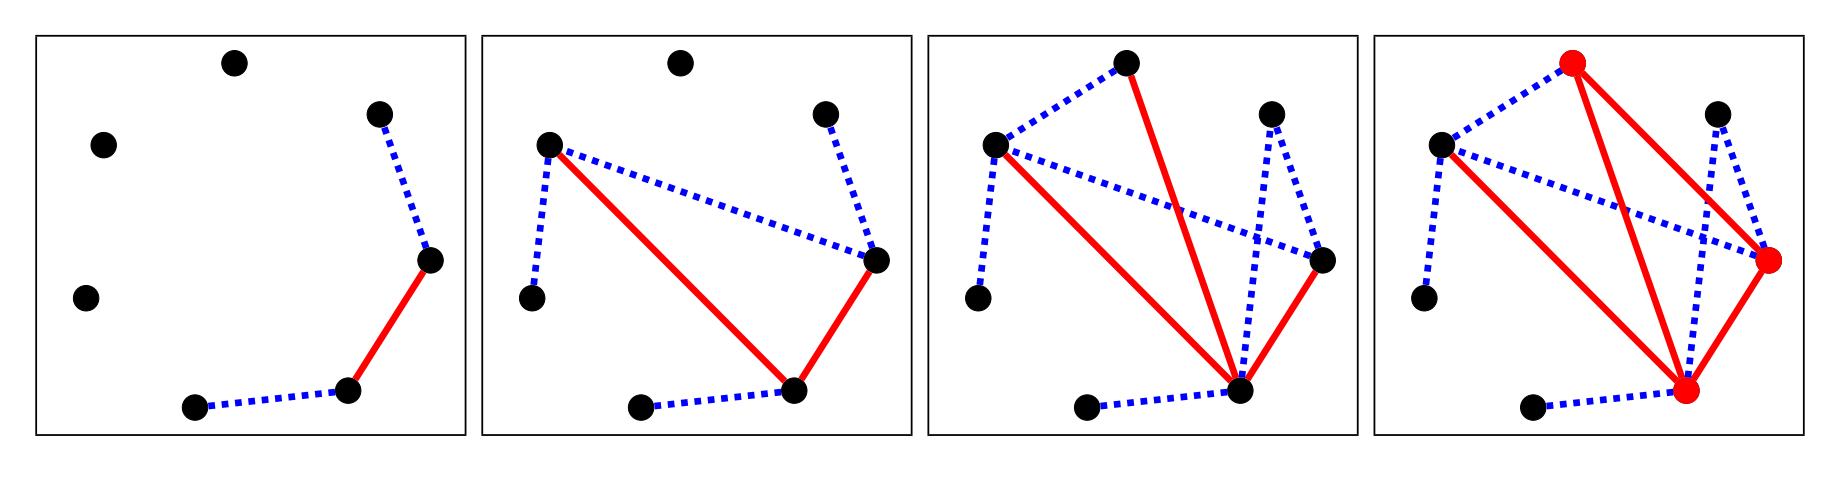
\includegraphics[width=14cm]{Maker Breaker image.png}
    \caption{The (7,2)-triangle game, $\textbf{G}(K_3;7,2)$, is a \textit{Maker}'s win. \textit{Maker}-edges are red, \textit{Breaker}-edges are blue. Image taken from \cite{glazik2022new}.}
    \label{fig:my_label}
\end{figure}

It is clear that as $b$ increases, the task of stopping \textit{Maker} from claiming a copy of $K_3$ becomes easier. That is to say if \textit{Breaker} has a winning strategy in $\textbf{G}(K_3;n,b_h)$ then he also has a winning strategy in $\textbf{G}(K_3;n,b_h+k)$, for all $k \in \mathbb{N}$. \\

Similarly it is true that as $b$ decreases, the task of claiming a copy of $K_3$ becomes easier for \textit{Maker}. That is, if \textit{Maker} has a winning strategy in $\textbf{G}(K_3;n,b_l)$, then she also has a winning strategy in $\textbf{G}(K_3;n,b_l-k)$, for all $k \in \mathbb{N}$.\\

We begin by observing the fact that for sufficiently large $n$, we have some non-trivial bounds on $b^*$ for the triangle game, that are functions of $n$.\\

We say that the game $\textbf{G}(G;n,b)$ is at round $t \in \mathbb{N}$ if either \textit{Maker} has claimed exactly $t-1$ edges and it is her turn, or \textit{Maker} has claimed exactly $t$ edges and it is \textit{Breaker}'s turn. In the first case we say $\textbf{G}(G;n,b)$ is at the start of round $t$ and in the second case we say $\textbf{G}(G;n,b)$ is at the end of round $t$. \\

Consider the following definition.

\begin{definition}[winning edge]

For the game $\textbf{G}(G;n,b)$ at the end of round $t$, a given unclaimed edge $uv \in E(K_n)$ is a winning edge if, by claiming it, \textit{Maker} would claim a copy of $G$.

\end{definition}

We now give a proof for the existence of some particular non-trivial bounds on $b^*$ for the $K_3$ \textit{Maker}-\textit{Breaker} game, first given by Chvátal and Erdős.

\begin{theorem}[Chvátal and Erdős \cite{chvatal1978biased}]{\label{6}}

If $b < \sqrt{2n+2} - 5/2$ then \textit{Maker} has a winning strategy for $\textbf{G}(K_3;n,b)$. On the other hand, if $b \geqslant 2\sqrt{n}$ then \textit{Breaker} has a winning strategy. 

\end{theorem}

We will first give Chvátal and Erdős' proof that if $b < \sqrt{2n+2}-5/2$, \textit{Maker} has a winning strategy in $\textbf{G}(K_3;n,b)$.

\begin{proof}

For $b < \sqrt{2n+2}-5/2$, we claim the following strategy wins for \textit{Maker} in $\textbf{G}(K_3;n,b)$.\\

\textit{Maker} starts the game and picks an arbitrary vertex $u \in V(K_n)$. \textit{Maker} will only claim edges at $u$ unless she has a chance to claim an edge that wins her the game, in which case she will deviate and claim it.\\

Suppose for a contradiction this strategy does not win. Then at the end of some round $t_1$, \textit{Maker} will have claimed $t_1$ edges of form $uv$. \textit{Breaker} will have claimed all remaining $n-1-t_1$ edges at $u$ and also the $t_1(t_1-1)/2$ edges between the $t_1$ vertices adjacent to $u$ claimed by \textit{Maker}.\\

Hence we have
\begin{equation}    
(n-1-t_1)+t_1(t_1-1)/2 \leqslant (t_1+1)b \,. \label{X}\end{equation}

Rearranging yields \[t_1^2+(-2b-3)t_1+2n-2-2b \leqslant 0 \, ,\]and taking the discriminant implies a solution does not exist for \[4b^2+20b-8n+17<0 \, ,\] which is the case when \[b < \sqrt{2n+2} - 5/2 \, ,\] and this is a contradiction.

\end{proof}

Now we will present Chvátal and Erdős' proof that if $b \geqslant 2\sqrt{n}$, \textit{Breaker} has a winning strategy in $\textbf{G}(K_3;n,b)$.

\begin{proof}
For $b \geqslant 2\sqrt{n}$, we claim the following strategy wins for \textit{Breaker} in $\textbf{G}(K_3;n,b)$.\\ 

Suppose \textit{Maker} claims some edge $uv$. Then \textit{Breaker} claims $ \lfloor \sqrt{n} \rfloor $ edges at $u$ and $ \lfloor \sqrt{n} \rfloor $ edges at $v$. If \textit{Breaker} cannot achieve this, he claims as many edges as possible at $u$ and $v$.\\

We claim that under this strategy, \textit{Maker} never claims more than $ \lfloor \sqrt{n} \rfloor + 1 $ edges claimed at any given vertex $w$. This follows from the fact that if \textit{Maker} has claimed $ \lfloor \sqrt{n} \rfloor +1 $ edges at $w$ at the start of some round $t$, then under this strategy \textit{Breaker} has claimed exactly $ \lfloor \sqrt{n} \rfloor^2$ edges at $w$ . So together \textit{Maker} and \textit{Breaker} have claimed  $ \lfloor \sqrt{n} \rfloor^2+\lfloor \sqrt{n} \rfloor +1 $ edges at $w$, which is strictly bounded below by $n-\sqrt{n}+1$ since, \[\lfloor \sqrt{n} \rfloor^2+\lfloor \sqrt{n} \rfloor +1>(\sqrt{n}-1)^2+\sqrt{n}-1+1=n-\sqrt{n}+1  \, .\] Hence \textit{Breaker} will proceed to claim all remaining edges at $w$ at the end of round $t$, since there are less then $\sqrt{n}-2 < \lfloor \sqrt{n} \rfloor$ unclaimed edges remaining. Hence at the beginning of round $t+1$ both players have collectively claimed all edges from $w$, and so \textit{Maker} cannot claim anymore than $ \lfloor \sqrt{n} \rfloor + 1 $ edges at $w$.\\

We now sophisticate \textit{Breaker}'s strategy by stating that he must also claim any winning edges when possible.\\

If \textit{Maker} cannot complete a triangle at the start of some round $t$, then if she is able to at the start of round $t+1$ it must be the case that if she claimed the edge $uv$ in round $t$, then any new winning edge must be of form $uw$ or $vx$. In either case there are at most  2$ \lfloor \sqrt{n} \rfloor $ possible such winning edges that may occur from the previous part, since they must contain one of the vertices of the edge claimed by \textit{Maker} during round $t$.\\

Hence \textit{Breaker} is able to claim all winning edges whenever they occur. By induction it follows that \textit{Maker} is never able to claim a winning edge, hence she is never able to claim a copy of $K_3$. Therefore \textit{Breaker} wins under this strategy. This strategy is executable provided $b \geqslant 2\lfloor \sqrt{n} \rfloor$, or provided $b \geqslant 2\sqrt{n}\,.$

\end{proof}

A point that should be noted is that the right-hand side of \eqref{X} is equal to $(t_1+1)b$ rather than $(t_1+0)b$. This is due to the fact that in the original paper by Chvátal and Erdős \cite{chvatal1978biased}, the game was played under the convention that it does not matter who gets the first move, so in letting \textit{Breaker} move first we are constructing a winning strategy for \textit{Maker} in a ``worst-case'' scenario.\\

In terms of the critical value, Theorem \ref{6} tells us that for $n$ sufficiently large (in fact in this instance for any n) it must be the case that for the game $\textbf{G}(K_3;n,b)$ we have that $\sqrt{2n+2}-5/2 < b^* < 2\sqrt{n}\,.$ We will come back to this idea of bounding $b^*$ later where we will bring up an important conjecture first given by Bednarska and \L{}uczak \cite{bednarska2000biased}.\\ 

Another idea in the above proof that is of particular interest is that for \textit{Breaker}'s strategy, when he wins, we see that he picks some of his edges arbitrarily. We will see in the next chapter that by sophisticating his strategy and picking his edges more carefully, he is able to improve on this upper bound. 

\chapter{Improving \textit{Breaker}'s Bounds}

Following from the previous chapter, it can be shown that under a more sophisticated strategy, \textit{Breaker} is able to win the game under the following stronger conditions. 

\begin{theorem}[Glazik and Srivastav \cite{glazik2022new}]\label{Glaik}

For sufficiently large n, if $b \geqslant \sqrt[]{(8/3 + o(1))n}$, then \textit{Breaker} has a winning strategy in $\textbf{G}(K_3;n,b)$.
    
\end{theorem}

Glazik and Srivastav improved on Chvátal and Erdős \textit{Breaker} bound in the triangle game through complicating \textit{Breaker}'s procedure for picking edges incident to the vertices claimed by \textit{Maker} on the previous turn. Compared to the Chvátal-Erdős \textit{Breaker} strategy of claiming some edges adjacent to the vertices previously claimed by \textit{Maker} arbitrarily, the Glazik-Srivastav \textit{Breaker} strategy has \textit{Breaker} claim edges adjacent to vertices previously claimed by \textit{Maker} in such a way that prioritises the ``most dangerous'' edges. That is, edges adjacent to vertices where \textit{Maker} had already claimed a relatively high proportion of edges, in comparison to \textit{Breaker}.\\

Consider an optimal \textit{Breaker} strategy. If, at some round $t$, \textit{Maker} is able to build some path $uvw$ of length 2, then if \textit{Breaker} has not claimed the edge $uw$ before the beginning of round $t+1$, \textit{Maker} will claim it at the beginning of round $t+1$ and win. This important fact means that in this situation, an optimal \textit{Breaker} strategy demands that if not previously claimed, \textit{Breaker} must claim the edge $uw$ in round $t$. From this, we can deduce that if \textit{Maker} is able to win the triangle game it necessitates that she is able to construct strictly more than $b$ paths of length 2 in a single round.\\

We now give a brief overview of the machinery of the Glazik-Srivastav strategy.\\

Let $\epsilon^* > 0$ and $\beta = \frac{8}{3}+\epsilon^*$. Assume $\beta \leqslant 4$ and fix $\delta \in (0,1-\frac{8}{3\beta})$. \\

\begin{definition}[balance]

    For every $v \in V(K_n)$, we define the balance of $v$, denoted $bal(v)$, as \[bal(v) = \frac{8(n-\deg_B(v))}{b^2(1-\delta)(3+\delta)-4\deg_M(v)(2b-\deg_M(v))}\, ,\]where $b$ is the maximum number of edges \textit{Breaker} can claim per round, $\deg_B(v)$ is the degree of $v$ in the subgraph constructed by \textit{Breaker}, and $\deg_M(v)$ is the degree of $v$ in the subgraph constructed by \textit{Maker}.
    
\end{definition}

We will not delve too deeply into the exact derivation of the definition. Note however that the balance of $v$ increases as $\deg_M(v)$ increases and decreases as $\deg_B(v)$ increases. That is to say the balance function gives us some sort of measure of how ``dangerous'' a vertex is. This allows \textit{Breaker} to put a relevant ordering on the vertices, which dictates how he picks his edges in each round, compared to the arbitrary element in the strategy of Chvátal and Erdős.\\

The final two tools used in \cite{glazik2022new} are the deficit and the potential function.

\begin{definition}[deficit]

    For every $v \in V(K_n)$, we define the deficit of $v$, denoted $d(v)$ as \[d(v) = \deg^*(v)-\deg_B(v)\,.\] Where $\deg^*(v)$ is the balanced \textit{Breaker} degree of $v$.
    
\end{definition}

A quick note on what a balanced \textit{Breaker} degree is. In the Glazik-Srivastav strategy, \textit{Breaker} is trying to keep the balance of a given vertex low. The balanced \textit{Breaker} degree of a vertex is the degree required in \textit{Breaker}'s subgraph to achieve a given real-valued balance. In Glasik and Srivastav's paper this given real-valued balance is an appropriate function of $n$, $b$, and $\delta$. We can see the deficit function as a way of measuring how far off \textit{Breaker} is from achieving a safe vertex and hence dictates when he needs to react.\\

Finally we consider the potential function. Let $\mu = 1 + \frac{6\beta \ln(n)}{\delta b}$.

\begin{definition}[potential]

For every $v \in V$, we define the potential of $v$, denoted pot($v$), as:

\[\text{pot}(v)=\left\{
    \begin{array}{lr}
        $0$ & \text{if } $\text{deg}_M(v) + \text{deg}_B(v)=n-1$\\
        $\mu^{d(v)/b}$ & \text{otherwise~~~~~~~~~~~~~~~~~~~~~~~~~~~} 
    \end{array}\,.\]

\end{definition}

 We can interpret the potential function as the main machinery of the proof. It once again measures the ``danger'' of a vertex and has an arguably more complex form than that of the balance or the deficit. This allows for the execution of the proof of a written deterministic strategy.\\

 The key takeaway from this chapter is that all 3 of these definitions (balance, deficit, and potential) measure the ``danger'' of any given vertex, a fundamental tool in aiding \textit{Breaker}'s attempt to play optimally. Each of these functions are increasing in \textit{Maker}'s degree and decreasing in \textit{Breaker}'s degree, intuitively what we would expect to be a natural candidate for a ``danger'' measure.\\
 
 We also note that Glazik and Srivatav's proof allows for some potential room for improvement, as they impose a very restricting strategy in which $b$ is picked such that in $\textbf{G}(K_3;n,b)$, \textit{Breaker} uses a winning strategy where he prevents \textit{Maker} from ever building a $\frac{b}{2}$ star. This is likely unnecessary for an optimal strategy and, if it is a necessary requirement for an optimal strategy, is almost certainly non-trivial to prove.
 
\chapter{Bounding the Critical Value for a General Game} 

We introduce a powerful result, first given by Bednarska and \L{}uczak, which we will use in the next chapter to provide a new result.

\begin{theorem}[Bednarska and \L{}uczak \cite{bednarska2000biased}]\label{1}

For every graph G that contains at least 3 non-isolated vertices, there exist positive constants $c_0$, $C_0$, and $n_0$ such that for every n with $n \geqslant n_0$, the following holds.

\begin{enumerate}
    
    \item If $b \leqslant c_0n^{1/m(G)}$, then \textit{Maker} has a winning strategy in the game $\textbf{G}(G;n,b)$.
    
    \item If $b \geqslant C_0n^{1/m(G)}$, then \textit{Breaker} has a winning strategy in the game $\textbf{G}(G;n,b)$.

\end{enumerate}

In the above, \[m(G)=\max\Big\{\frac{e(H)-1}{v(H)-2}:H\subseteq{G} \text{ and } v(H) \geqslant 3\Big\}\,.\]

\end{theorem}

Theorem \ref{1} is helpful as we are mainly concerned with the outcome of the game $\textbf{G}(G;n,b)$ for sufficiently large $n$. Furthermore, since Theorem \ref{1} applies to all complete graphs on $m \geqslant 3$ vertices, then we may use this to immediately generate the right ``order'' of the bounds for any clique game,  $\textbf{G}(K_m;n,b)$. Note that for a complete graph of order $m$ greater than or equal to $3$, the value of $m(G) = \frac{\binom{m}{2}-1}{m-2} = \frac{m+1}{2}$. That is to say it is easy to calculate $m(G)$ when $G = K_m$ for some integer $m \geqslant 3$.\\

A full proof of Theorem \ref{1} can be found in Bednarska and \L{}uczak's original paper \cite{bednarska2000biased}. A brief overview of the technique is as follows.\\

We first begin with covering the general idea behind proving the \textit{Maker} bound, which uses a probabilistic ``derandomization'' argument. Consider a modification of the game $\textbf{G}(G;n,b)$ denoted  $\overline{\textbf{G}}(G;n,b)$ as follows.

\begin{definition}[blind \textit{Maker}-\textit{Breaker} game]

For $n$ a natural number and $b$ a non-negative integer, let $\overline{\textbf{G}}(G;n,b)$ denote the modified \textit{Maker}-\textit{Breaker} game in which \textit{Maker} chooses which edges she is going to claim in each round prior to the game. If at any point \textit{Maker} is unable to execute her move, due to \textit{Breaker} already claiming the edge she wanted, she will skip her turn and not claim any edge. \textit{Maker} wins if she is able to claim a copy of $G$. \textit{Breaker} wins otherwise.
    
\end{definition}

We now impose that \textit{Maker} will play $\overline{\textbf{G}}(G;n,b)$ according to a random strategy. That is, when selecting which edges she is going to claim in each round prior to the game, she does so in such a way that at each round she claims uniformly at random an edge previously unclaimed by herself. Note that if \textit{Breaker} has a winning strategy in $\textbf{G}(G;n,b)$ then he certainly has a winning strategy in $\overline{\textbf{G}}(G;n,b)$. Hence if \textit{Maker} can win the game $\overline{\textbf{G}}(G;n,b)$ then she has a winning strategy in $\textbf{G}(G;n,b)$. That is to say, if we can show that under a random strategy, with some positive probability, \textit{Maker} is able to win  the game $\overline{\textbf{G}}(G;n,b)$, then she must have a winning strategy in $\textbf{G}(G;n,b)$.\\

An important observation here is that in order to show that under a random strategy, \textit{Maker} has some positive probability of winning $\overline{\textbf{G}}(G;n,b)$, we really would like to know the answer to the following question. \[\textit{For a random graph }\mathbb{G}(n,p) \textit{ what is the probability there is a copy of } H \textit{ in } \mathbb{G}(n,p) \text{?}  \]

Where $\mathbb{G}(n,p)$ is the random graph generated on $n$ vertices where for every edge $uv \in E(K_n)$ there is a probability $p$ that it is in $E(\mathbb{G}(n,p))$.\\

In Bednarska and \L{}uczak's paper, they use the following lemma.

\begin{lemma}[Janson, \L{}uczak and Ruci\'{n}ski \cite{janson1990exponential}] \label{2}

For every graph $G$ containing a cycle there exist constants $c_1 > 0$ and $n_1$, such that for every $n \geqslant n_1$ and $n^{-1/m(G)} \leqslant p \leqslant 3n^{-1/m(G)}\,,$ \[\mathbb{P}(\mathbb{G}(n,p) \not\supseteq G) \leqslant \exp(-c_1n^2p)\,.\]  

\end{lemma}

The remainder of the proof revolves around manipulating Lemma \ref{2}. The key idea is that we can deduce from Lemma \ref{2} a lower bound on the probability that for a suitably large subgraph $D$ in the random graph $\mathbb{G}(n,M)$, the probability $D$ contains a copy of $G$. Here $\mathbb{G}(n,M)$ denotes the random graph on $n$ vertices with $M$ distinct edges picked uniformly from the set $\binom{[n]}{2}$. \\

For an appropriate choice of $b$, Bednarska and \L{}uczak show that with some positive probability, where $n$ is sufficiently large, the number of suitably large subgraphs $D$ in \textit{Maker}'s random graph which contain a copy of $G$ at some round $t$ exceeds the number of edges needed by \textit{Breaker} to interfere with each and every one of them at that round. Hence at some round of the game \textit{Maker} has a positive probability of claiming a copy of $G$ in the game $\overline{\textbf{G}}(G;n,b)$. Thus she has some winning strategy in $\textbf{G}(G;n,b)$. \\

Now we discuss the key ideas used in proving the \textit{Breaker} bound. Bednarska and \L{}uczak proved that \textit{Breaker} has a winning strategy in ${\textbf{G}}(G;n,b)$, for suitably chosen $b$, using a deterministic approach, rather than a probabilistic one used in proving the \textit{Maker} bound.\\

We first introduce the concept of a hypergraph.

\begin{definition}[hypergraph]

A hypergraph $\mathcal{G}$ is defined as a pair of sets $(V,\mathcal{E})$ where $V$ is the set of vertices of $\mathcal{G}$ and $\mathcal{E}$ is the set of edges of $\mathcal{G}$ such that $\mathcal{E} \subseteq 2^V$.
    
\end{definition}

Observe here that all graphs considered in this dissertation so far are in fact also hypergraphs, so any result that we know applies to hypergraphs will also be applicable to these ``standard graphs'', also known as $2$-graphs.\\

Hence we are able to apply the following theorem, proven by Beck.\\

First define $\textbf{G}(\mathcal{G};a,b)$ to be the biased hypergraph \textit{Maker}-\textit{Breaker} game in which \textit{Maker} and \textit{Breaker} alternatively claim $a$ and $b$ edges of $V$ respectively until all vertices have been claimed by either player. If at the end of the game \textit{Maker} has claimed all vertices of some $A \in \mathcal{E}$, she wins. Otherwise \textit{Breaker} wins. Then we have,

\begin{theorem}[Beck \cite{beck1982remarks}]\label{3}

For $\textbf{G}(\mathcal{G};a,b)$ let \[f(\mathcal{G}, a, b) = \sum_{A \in \mathcal{E}}(1+b)^{-\lvert A \rvert/a}\,.\] Then if $f(\mathcal{G},a,b) < (1+b)^{-1}$ \textit{Breaker} has a winning strategy, in such a way that the function \[g(M,B) = \sum_{\substack{A \in \mathcal{E} \\ A \cap B = \emptyset}}(1+b)^{-\lvert A \backslash M \rvert / a}\,,\] where $M$ and $B$ denote the vertex set's of \textit{Maker} and \textit{Breaker} respectively, never increases if it is evaluated after every move of \textit{Maker}.

\end{theorem}

Note here the function $g(M,B)$ has the trait that it gives a measure of ``danger''. Increasing the cardinality of $B$ will never increase $g(M,B)$ whereas increasing the cardinality of $M$ will never decrease $g(M,B)$.\\

The second idea used in the proof is that we need only prove that Theorem \ref{1} holds for graphs that are $m$-maximal. We call a graph $m$-maximal if it satisfies the following definition.

\begin{definition}[$m$-maximal]

A graph $G$ is $m$-maximal if, \[m(G) = \frac{e(G)-1}{v(G)-2} > m(H) \text{ for all } H \subset G \text{ such that } v(H) \geqslant 3\,,\]

where $m(G)$ is defined in Theorem \ref{1}.
    
\end{definition}

We need only prove Theorem \ref{1} holds for $m$-maximal graphs since suppose we have some $H$ which is $m$-maximal. Then if \textit{Breaker} has a winning strategy for the game $\textbf{G}(H;n,b)$, he can use the same strategy to win $\textbf{G}(G;n,b)$, provided that $H \subseteq G$, whilst simultaneously matching the correct order of $n$ required by Theorem \ref{1}.\\

The rest of the proof relies on a similar motif used in both previous chapters in giving a \textit{Breaker} bound, in which we show that \textit{Breaker} is able to limit the number of winning edges \textit{Maker} can posses at the end of each round. If we can bound this by the \textit{Breaker} bias $b$ then it suffices in proving \textit{Breaker} has a winning strategy in $\textbf{G}(G;n,b)$. This is achievable by playing the strategy mentioned in Theorem \ref{3} to give two strategies that \textit{Breaker} can execute simultaneously such that \textit{Maker} can never claim a dangerous $q$-fan of appropriate size. A $q$-fan is defined as follows.

\begin{definition}[$q$-fan]

For an $m$-maximal graph $G$ we denote a $\hat{G}$-graph $F^{v,w}$ as a graph $F$ such that $F + vw = G$ and $vw \notin E(F)$. Let $\mathbb{F} = \{F_1^{v_1,w_1}, \ldots , F_t^{v_q,w_q} \}$ be a family of $q$ different $\hat{G}$-graphs. If $\lvert \bigcap_{i=1}^q V(F_i^{v_i,w_i}) \rvert \geqslant 2$ we call a family $\mathbb{F}$ a $q$-fan. 

\end{definition}

Following on we have that a dangerous $q$-fan is defined as,

\begin{definition}[dangerous $q$-fan]
    If at any moment of the game  $\textbf{G}(G;n,b)$ \textit{Maker} has a $q$-fan which consists of $q$ distinct $\hat{G}$-graphs, such that for each  $\hat{G}$-graph $F^{v_i,w_i}$ forming the $q$-fan, the edge $v_iw_i$ has not been claimed by \textit{Breaker}, then we say this is a dangerous $q$-fan.
\end{definition}

Next we have the following lemma, \cite[Lemma~9]{bednarska2000biased}, which we will omit the proof of.

\begin{lemma}[Bednarska and \L{}uczak \cite{bednarska2000biased}]\label{LemmaBedna}

For every $m$-maximal graph $G$ that contains a cycle there exist constants $C_3$ and $n_3$ such that for every $n \geqslant n_3$ and $b \geqslant C_3n^{1/m(G)}$ where $m(G)$ is the function defined in Theorem \ref{1}, \textit{Breaker} has a strategy such that at no stage of the game $\textbf{G}(G;n,b)$ \textit{Maker}'s graph contains a dangerous $b$-fan.

\end{lemma}

From this, we can prove Theorem \ref{1}. For the case that $G$ is not a forest (if $G$ is a forest Theorem \ref{1} holds trivially) we have the following.\\

From Lemma \ref{LemmaBedna}, setting $2C_0 = C_3$, with $b \geqslant C_0n^{1/m(G)}$, and $C_3$ satisfying the conditions set out in Lemma \ref{LemmaBedna}, we have that in the game $\textbf{G}(G;n,b/2)$ \textit{Breaker} has a strategy such that \textit{Maker} can never claim a dangerous $b/2$-fan provided $n$ is sufficiently large. We now consider the original game $\textbf{G}(G;n,b)$.\\

If \textit{Maker} is able to win the game $\textbf{G}(G;n,b)$ it must be the case that at some point of the game, she possesses a $\hat{G}$-graph $F^{v,w}$ in which the edge $vw$ has not been claimed by \textit{Breaker}.\\

Then in $\textbf{G}(G;n,b)$ \textit{Breaker} wins with the following strategy. At each turn he will use $b/2$ edges to execute the strategy in the game  $\textbf{G}(G;n,b/2)$ such that \textit{Maker} will never claim a dangerous $b/2$-fan.\\

Consider \textit{Maker}'s last move immediately before \textit{Breaker}'s. Any new dangerous $\hat{G}$-graph claimed by \textit{Maker} must contain the last edge she claimed. Hence, any new dangerous $\hat{G}$-graph must take the form of a dangerous $q$-fan, with $q < b/2$. Hence \textit{Breaker} is able to use his remaining $b/2$ edges to claim all new winning edges created by \textit{Maker}. Therefore \textit{Breaker} is able to always claim any winning edge created by \textit{Maker} each turn, verifying he has a winning strategy in $\textbf{G}(G;n,b)$. \\

The technical details for both proving the \textit{Maker} and \textit{Breaker} bounds are quite long as aforementioned, and I point the reader to the original paper for full details of these proofs. Note however the difference in proof techniques, namely that the \textit{Maker} bound relies on a probabilistic approach, whereas the \textit{Breaker} bound can be proven deterministically.\\

It is possibly for this reason that \textit{Maker} bounds are usually harder to prove compared to \textit{Breaker} bounds. (Indeed at the time of submission, if we look at the majority of the literature for the triangle game, we see that outside of Chvátal and Erdős' original bound on \textit{Maker}'s winning strategy, there have been no new papers on improving \textit{Maker}'s bound.)\\

We conclude this chapter by mentioning a key conjecture.

\begin{conjecture}[Bednarska and \L{}uczak \cite{bednarska2000biased}]\label{Conjecture}
For every graph $G$ and $\epsilon>0$, there exists a constant $c>0$ and a natural number $n_0$ such that for every $n \geqslant n_0$ the following holds.

\begin{enumerate}
    
    \item If $b \leqslant (c-\epsilon)n^{1/m(G)}$, then \textit{Maker} has a winning strategy in the game $\textbf{G}(G;n,b)$.
    
    \item If $b \geqslant (c+\epsilon)n^{1/m(G)}$, then \textit{Breaker} has a winning strategy in the game $\textbf{G}(G;n,b)$.

\end{enumerate}
\end{conjecture}

Conjecture \ref{Conjecture} remains open to prove for any graph $G$ which contains a cycle.

\chapter{The $K_4$ \textit{Maker}-\textit{Breaker} Game and Non-Trivial Bounds}

We will now prove a new result that gives us some non-trivial bounds on the value of $b^*$ for the game $\textbf{G}(K_4;n,b)$.
This is the game played on $K_n$ except unlike before in the triangle game, \textit{Maker} is now trying to construct a copy of $K_4$ rather than a copy of $K_3$. \\

Before a formal proof is given, we first describe the strategy of obtaining these bounds. We effectively reverse engineer the proof of Theorem \ref{1} in order to obtain the relevant constants. This requires the use of a few more results, not covered in enough detail to give explicit numerical bounds in Bednarska and \L{}uczak's original paper, which we will present in sufficient detail in our proof here.\\

From Theorem \ref{1} we have the following corollary. 

\begin{corollary}

There exist positive constants $a_0$ and $A_0$ such that for $n$ sufficiently large,

\begin{enumerate}
    
    \item If $b \leqslant a_0n^{2/5}$, then \textit{Maker} has a winning strategy in the game $\textbf{G}(K_4;n,b)\,.$ 
    
    \item If $b \geqslant A_0n^{2/5}$, then \textit{Breaker} has a winning strategy in the game $\textbf{G}(K_4;n,b)\,.$

\end{enumerate}
    
\end{corollary}

We will first give a non-trivial numerical value for a valid \textit{Maker} constant \[a_0 = 0.0001 \,.\]

\begin{theorem}{\label{4}}

     If $b \leqslant 0.0001n^{2/5}$ and $n$ is sufficiently large, \textit{Maker} has a winning strategy in the game $\textbf{G}(K_4;n,b)$.
     
\end{theorem}

\begin{proof}

Let $\alpha$ and $\beta$ be arbitrary sets (not necessarily distinct) consisting of exactly 4 vertices in $[n]$. Set $\alpha \sim \beta$ if and only if $\lvert \alpha \cap \beta \rvert \geqslant 2$, and for $\gamma \in \{\alpha, \beta\}$, set $\mathbbm{1}_{\gamma}$ to be the indicator function which equals $1$ if the induced subgraph on $\gamma$ in  $\mathbb{G}(n,p)$ is a copy of $K_4$ and equals $0$ otherwise. Then from \cite[Lemma~1]{janson1990exponential}, we have that,  \[\log(\mathbb{P}(\mathbb{G}(n,p) \not\supseteq K_4)) \leqslant -\sum_\alpha \mathbb{E}\Big{[}\frac{\mathbbm{1}_{\{\alpha\}}}{\sum_{\alpha \sim \beta} \mathbbm{1}_{\{\beta\}}}\Big{]}\,,\] where we are summing over all possible $\alpha \in \binom{[n]}{4}$.\\

Rearranging and evaluating the right hand side of the inequality, interpreting 0/0 as 0, we have that,
\begin{flalign*}
-\sum_\alpha \mathbb{E}\Big{[}\frac{\mathbbm{1}_{\{\alpha\}}}{\sum_{\alpha \sim \beta}\mathbbm{1}_{\{\beta\}}}\Big{]} & = -\sum_\alpha \mathbb{E}\Big{[}\mathbb{P}(\mathbbm{1}_{\{\alpha\}}=1) \frac{1}{\sum_{\alpha \sim \beta}\mathbbm{1}_{\{\beta\}}} | \mathbbm{1}_{\{\alpha\}}=1\Big{]}&\\
     & =-\mathbb{P}(\mathbbm{1}_{\{\alpha\}}=1)\sum_\alpha \mathbb{E}\Big{[}\frac{1}{\sum_{\alpha \sim \beta}\mathbbm{1}_{\{\beta\}}} | \mathbbm{1}_{\{\alpha\}}=1\Big{]}&\\
     & =-p^6 \binom{n}{4} \frac{1}{1+ \binom{4}{3}\binom{n-4}{1}p^3+\binom{4}{2}\binom{n-4}{2}p^5}&\\
     &=-\frac{(n^4-6n^3+11n^2-6n)p^6}{72n^2p^5-648np^5+1440p^5+96np^3-384p^3+24}&\\
     &\leqslant -\frac{1}{72+\epsilon}n^2p \,.
\end{flalign*}

for $n$ sufficiently large, $\epsilon>0$, and $n^{-2/5} \leqslant p \leqslant 3n^{-2/5}$.\\

That is to say, for $n$ sufficiently large, $\epsilon>0$, and $n^{-2/5} \leqslant p \leqslant 3n^{-2/5}$ we have that  \[\mathbb{P}(\mathbb{G}(n,p) \not\supseteq K_4) \leqslant \exp(-\Big{(}\frac{1}{72+\epsilon}\Big{)}n^2p)\,. \]

We will now use the following lemma, \cite[Lemma~1.2]{frieze2016introduction}.

\begin{lemma}\label{7}

    Let $\mathcal{P}$ be any subset of the set of all labelled graphs on vertex set $[n]$ and $p = \frac{m}{\binom{n}{2}}$, where as $n \rightarrow \infty$ we have $m=m(n) \rightarrow \infty$, and $\binom{n}{2}-m \rightarrow \infty$. Then for $n$ sufficiently large, \[\mathbb{P}(\mathbb{G}(n,m) \in \mathcal{P}) \leqslant 10m^{1/2}\mathbb{P}(\mathbb{G}(n,p) \in \mathcal{P})\,.\]
    
\end{lemma}

Setting $\mathcal{P}$ to be the set of all graphs on $n$ vertices which do not contain a copy of $K_4$, $\overline{M} = m = m(n) = \lfloor n^{8/5} \rfloor$, $p = \frac{\overline{M}}{\binom{n}{2}}$, and taking $n$ sufficiently large, we are able to apply Lemma \ref{7}.\\

We have, 
\begin{flalign*}
~~~~~~~~~~~~~~~~~~~\mathbb{P}(\mathbb{G}(n,\overline{M}) \not\supseteq K_4)&  = \mathbb{P}(\mathbb{G}(n,\overline{M}) \in \mathcal{P})&\\
     & \leqslant 10 \overline{M}^{1/2} (\mathbb{P}(\mathbb{G}(n,p)) \in \mathcal{P})&\\
     & =10\overline{M}^{1/2}(\mathbb{P}(\mathbb{G}(n,p) \not\supseteq K_4))&\\
     &\leqslant 10\overline{M}^{1/2} \exp(-\frac{1}{72+\epsilon}n^2p)&\\
     &=10 \lfloor n^{8/5} \rfloor^{\frac{1}{2}}\exp(-\frac{1}{72+\epsilon}n^2p)&\\
     &\leqslant \exp(-\frac{1}{72+2\epsilon}n^2p)&\\
     &=\exp(-\frac{1}{72+2\epsilon}n^2\frac{\lfloor n^{8/5} \rfloor}{\binom{n}{2}})&\\
     &\leqslant \exp((-\frac{2}{72+2\epsilon})\overline{M})\,.
    \end{flalign*}

So we have that in \cite[Lemma~$3^\prime$]{bednarska2000biased}, we can pick, \[c_1^\prime = \frac{2}{72+2\epsilon}\,,\]such that $\mathbb{P}(\mathbb{G}(n,\overline{M}) \not\supseteq K_4) \leqslant \exp(-c_1^\prime \overline{M})$ where $\overline{M} = \lfloor n^{8/5} \rfloor$.\\

Solving now for $\delta$ from \cite[Lemma~4]{bednarska2000biased}, we have that for $0 < \delta =0.001 < 1/2$, \[\delta-\delta\log(\delta)=0.001-0.001\log(0.001)<\frac{2}{216}\,.\] Hence for $\epsilon$ sufficiently small, we have $\delta - \delta\log(\delta) < c_1^\prime/3$. It follows that from \cite[Proof~of~Theorem~2]{bednarska2000biased}, we have that for $b = 0.1\delta n^{2/5} = 0.0001 n^{2/5}$ and $n$ sufficiently large, \textit{Maker} has a winning strategy in the game $\textbf{G}(K_4;n,b)$, which verifies Theorem \ref{4}. 

\end{proof}

We will now give a non-trivial numerical value for a valid \textit{Breaker} constant, \[A_0 = 4(72e)^{1/5}+o(1)\,.\]

\begin{theorem}{\label{5}}
    
If $b \geqslant (4(72e)^{1/5}+o(1))n^{2/5}$ and $n$ is sufficiently large, then \textit{Breaker} has a winning strategy in the game $\textbf{G}(K_4;n,b)$.

\end{theorem}

\begin{proof}

Observe that $K_4$ is an $m$-maximal graph, hence we can work backwards directly from \cite[Lemma~7]{bednarska2000biased}. We have,

\begin{flalign*}
(b+1)\binom{n}{2}\frac{1}{t!}(v(K_4)!e(K_4)&\binom{n}{v(K_4)-2}(b+1)^{-e(K_4)+2})^t &\\& =(b+1)\binom{n}{2}\frac{1}{t!}(144\binom{n}{2}(b+1)^{-4})^t&\\
     & =\frac{72^t}{2t!}(n(n-1))^{t+1}(b+1)^{-4t+1}&\\
     & \leqslant\frac{72^t}{2t!}(n^2)^{t+1}b^{-4t+1}&\\
     &=\frac{1}{2t!}bn^2(72n^2b^{-4})^t&\\
     &\leqslant\frac{1}{2(2\pi t)^{1/2}(\frac{t}{e})^te^{\frac{1}{12t+1}}}bn^2(72n^2b^{-4})^t &\\
     &\leqslant\frac{1}{(\frac{t}{e})^t}bn^2(72en^2b^{-4})^t&\\
     &=bn^2(72en^2b^{-4}t^{-1})^t\,,
\end{flalign*}

where we have used a Stirling approximation to achieve the inequality in the third from bottom line of algebra above. This is the required form needed so that we can take out the constant, \[c_2 = 72e\,.\]
We now solve for two constants, $n_2$ and $C_2$, that satisfy
\[((72e)^{-1}(C_2)^5)^{b^{\frac{\delta}{3}}} > 2b^6\,,\]
where $0 < \delta <1$ and such that
\[b \geqslant C_2(n_2)^{2/5}\,.\]
Suppose 
\[(72e)^{-1}(C_2)^5>1 \,.\]
Then it follows trivially that there exists some constant $n_2$ sufficiently large such that the first inequality holds, as we can bound $b$ from below such that $b$ is sufficiently large. Hence we need,
\[C_2 > (72e)^{1/5} > 1 =C_1\,.\]
We have,
\[C_0 = 2C_3 = 4C_2 > 4(72e)^{1/5} \,,\]
which implies
\[C_0 \geqslant 4(72e)^{1/5}+o(1)\,,\]
which by \cite[Proof~of~Theorem~1(ii)]{bednarska2000biased} verifies Theorem \ref{5}.


\end{proof}

\chapter{A Practical Attempt at Winning for \textit{Maker} in Higher Clique Games}

In the previous chapter we gave new bounds for the critical value $b^*$ for the game $\textbf{G}(K_4;n,b)$, through showing the existence of two strategies, one for \textit{Maker} and one for \textit{Breaker}, which for appropriately chosen $b$ guarantee a win for each agent.\\

For \textit{Breaker} we were able to give an explicit, winning deterministic strategy, given in \cite{bednarska2000biased} and based of the strategy given in \cite{beck1982remarks}. On the other hand we were only able to prove the existence of a winning \textit{Maker} strategy through a probabilistic approach, without giving one explicitly.\\

The remainder of this chapter describes a strategy that is practically executable for \textit{Maker}, which allows her to win any game of the form $\textbf{G}(K_m;n,b)$, that is a clique \textit{Maker}-\textit{Breaker} game, provided the \textit{Breaker} bias $b$ is strictly less than some function $f(n)$, with $o(f(n)) = n^{g(m)}$, where $g(m)$ is some non-constant function of $m$, and $n$ is sufficiently large.\\

The strategy that \textit{Maker} will use is as follows.

\begin{definition}[The N-I attack]

The N-I attack (Neighbourhood-Independent Set attack) is a 2-stage strategy used by \textit{Maker} in the game $\textbf{G}(K_m;n,b)$, where $m$ is some natural number greater than or equal to 3. In stage 1, \textit{Maker} will claim a neighbourhood of sufficient size at some arbitrary vertex $v \in V(K_n)$. In stage 2, \textit{Maker} will then attempt to win the game $\textbf{G}(K_{m-1};s,b)$ on some independent set $S \subseteq N(v)$, where $\lvert S \rvert = s$.   

\end{definition}

Note that if \textit{Maker} is able to execute stage 2 of the N-I attack, that is she is able to win $\textbf{G}(K_{m-1};s,b)$ on $S$, then \textit{Maker} will have won $\textbf{G}(K_m;n,b)$. This follows since every vertex in the copy of $K_{m-1}$ she claimed in stage 2, shares an edge with the vertex $v \notin N(v)$, hence the induced subgraph on $K_{m-1}+\{v\}$ forms a copy of $K_m$.\\

We will now give a new theorem on the bounds for which the N-I attack is successful for \textit{Maker}.

\begin{theorem}\label{sodiumattack}

    For the game $\textbf{G}(K_m;n,b)$ where $m$ is a natural number at least 3 and $n$ is sufficiently large, the N-I attack will result in a win for \textit{Maker} if $b < \frac{1}{\sqrt{2}}\sqrt[2m-4]{2^{10-3m}}n^{\frac{1}{2m-4}}$.
    
\end{theorem}

    \begin{proof}
    
         We proceed by strong induction. For the case $m=3$ from Theorem \ref{6} and its proof of the \textit{Maker} bound, we have that the statement holds.\\

         Suppose that for some natural number $k$ greater than or equal to 3, Theorem \ref{sodiumattack} holds for all $m \leqslant k$.\\

     Consider $\textbf{G}(K_{k+1};n,b)$ and set $b \leqslant cn^{\frac{1}{2(k+1)-4}}\,.$ \textit{Maker} plays the N-I attack and claims some neighbourhood of $x$ of size $\lceil \frac{a}{c}n^{1-\frac{1}{2(k+1)-4}} \rceil$ where $a \in (0,1)$ and $x$ is an arbitrary vertex. This is possible since for $n$ sufficiently large, together \textit{Maker} and \textit{Breaker} claim less than $\lceil \frac{a}{c}n^{1-\frac{1}{2(k+1)-4}} \rceil + an < n-1$ edges at $x$ before the end of round $\lceil \frac{a}{c}n^{1-\frac{1}{2(k+1)-4}} \rceil$.\\

         Consider the neighbourhood of $x$ denoted $N(x)$. We call a vertex $v$ \textit{enormous} if the degree of $v$ in $N(x)_B$, that is the \textit{Breaker} degree of $v$ in $N(x)$, is greater than or equal to $dn^{\frac{1}{2(k+1)-4}}$ for some $d > 0$. Let $E$ denote the set of all \textit{enormous} vertices in $N(x)$. Then we must have $\lvert E \rvert < \frac{2}{d}n^{1-\frac{1}{2(k+1)-4}}$ at the start of round  $\lceil \frac{a}{c}n^{1-\frac{1}{2(k+1)-4}} \rceil+1$,  since \textit{Breaker} has claimed strictly less than $n$ edges in total, provided $n$ is sufficiently large.\\

         Consider the subgraph $G^{\prime} = N(x)-E$. We have that,\[\lvert G^{\prime} \rvert = \lvert N(x)-E \rvert > \frac{ad-2c}{cd}n^{1-\frac{1}{2(k+1)-4}}\,,\]and we have $\Delta(G^{\prime}) < dn^{\frac{1}{2(k+1)-4}}$, since we know any vertex in $V(G^{\prime})$ is not \textit{enormous}. Hence for $n$ sufficiently large, \[\alpha(G^{\prime}) > \frac{1}{2}\frac{ad-2c}{cd^2}n^{1-\frac{1}{(k+1)-2}}\,,\]where we are multiplying by $\frac{1}{2}$ to guarantee strict equality. (We really could use any positive constant less than $1$ here, and it would generate a different initial multiplier. In this case we get $\frac{1}{\sqrt{2}}$.) Consider some independence set of size $\lceil \frac{ad-2c}{2cd^2}n^{1-\frac{1}{(k+1)-2}} \rceil$ in $N(x)$ at the start of round $\lceil \frac{a}{c}n^{1-\frac{1}{2(k+1)-4}} \rceil+1$ which we know exists. Then from the induction hypothesis we have that provided, \[cn^{\frac{1}{2(k+1)-4}} < \frac{1}{\sqrt{2}}\sqrt[2k-4]{2^{10-3k}}(\lceil \frac{ad-2c}{2cd^2}n^{1-\frac{1}{(k+1)-2}} \rceil)^{\frac{1}{2k-4}}\,,\] \textit{Maker} is able to win  $\textbf{G}(K_k;\lceil \frac{ad-2c}{2cd^2}n^{1-\frac{1}{(k+1)-2}} \rceil,b)$, and hence win stage 2, which holds if for $n$ sufficiently large,\[cn^{\frac{1}{2(k+1)-4}} < \frac{1}{\sqrt{2}}\sqrt[2k-4]{2^{10-3k}}(\frac{ad-2c}{2cd^2}n^{1-\frac{1}{(k+1)-2}})^{\frac{1}{2k-4}}\,.\] Note that on both sides of the inequality, we have the same order of $n$, hence the inequality above holds if and only if, \[c < \frac{1}{\sqrt{2}}\sqrt[2k-4]{2^{10-3k}}(\frac{ad-2c}{2cd^2})^{\frac{1}{2k-4}}\,,\]which holds provided,\[ (2^{4k-11})c^{2k-3}d^2-d+2c<0\,,\]where we have taken $a$ arbitrarily close to 1. Taking the discriminant and noting the shape of the quadratic function in $d$ is centred to the right of the origin, we see the above equation has strictly positive solutions for $c$ and $d$ if and only if we have: \[1-4(2^{4k-11})c^{2k-3}2c > 0\,,\] which is the case when \[c < \sqrt[2k-2]{2^{8-4k}}=\frac{1}{\sqrt{2}}\sqrt[2(k+1)-4]{2^{10-3(k+1)}}\,,\]and this implies \textit{Maker} is able to win provided, \[b<\frac{1}{\sqrt{2}}\sqrt[2(k+1)-4]{2^{10-3(k+1)}}n^{\frac{1}{2(k+1)-4}}\,,\] verifying the induction step. By strong induction Theorem \ref{sodiumattack} holds.
            
         
    \end{proof}

We will finally note that in an optimal setting, this strategy is more or less redundant. From Theorem \ref{1}, for $m \neq 3$, we know that \textit{Maker} is able to win under much weaker restrictions on $b$, for sufficiently large $n$ having a certified win in $\textbf{G}(K_m;n,b)$ provided $b \leqslant m_0n^{\frac{2}{m+1}}$, where $m_0$ is some strictly positive constant.\\

The N-I attack demonstrates a key point made in \cite{bednarska2000biased}, in which Bednarska and {\L}uczak note that an optimal \textit{Maker} strategy requires her to play almost randomly. We see that by imposing strict rules, such as forcing \textit{Maker} to play on a neighbourhood of a single vertex, we do not obtain a strategy that immediately gives optimal bounds for \textit{Maker} in the game $\textbf{G}(K_m;n,b)$, where $m \geqslant 4$.

\chapter{Conclusion}

For the game $\textbf{G}(K_4;n,b)$, we have shown that for $n$ sufficiently large, the critical value $b^*$ satisfies:\[0.0001n^{2/5} \leqslant b^* < (4(72e)^{1/5}+o(1))n^{2/5}\,.\]We note that for our choice of $\delta$ in the proof of Theorem \ref{4}, we could have picked a slightly higher value to tighten the above bound, but only by a marginal amount. As expected, working backwards from the proof of Theorem \ref{1} has given us rather wide bounds on the critical value, and it would be interesting to see how tight this can be made in comparison to the best current bounds on the critical value for the game $\textbf{G}(K_3;n,b)$.\\

We also offer up the following conjecture:

\begin{conjecture}
    For all integers $m \geqslant 4$, there is no natural number $N$ with the property that for all $n \geqslant N$ a generalised neighbourhood attack allows for a \textit{Maker} win in $\textbf{G}(K_m;n,b)$, where $b \leqslant J_0n^{2/m+1}$, and $J_0$ is a fixed positive constant.
    
\end{conjecture}

Here a generalised neighbourhood attack describes the process of trying to claim a copy of $K_{m-1}$ on some neighbourhood $N(x)$ in order to claim a copy of $K_m$. That is we force \textit{Maker} to only claim edges at one vertex $x$ in her first $t_1$ moves and then for the rest of the game only ever claim edges in $N(x)$.\\

In our initial attempt to solve for some $K_4$ critical bounds, this was the attempted strategy, but typically it failed to derive a non-trivial bound of order $n^{2/5}$. If this conjecture is true, a very interesting observation is that for $m = 3$ the generalised neighbourhood attack does indeed work, as shown in the proof of Theorem \ref{6}, whilst also achieving the optimality bounds described by Theorem \ref{1}. A possible reason for this is that \textit{Maker} can immediately start generating winning edges using a generalised neighbourhood attack in $\textbf{G}(K_3;n,b)$, which is not the case for any higher clique game. This means that an optimal \textit{Breaker} strategy does not necessarily demand he react immediately to \textit{Maker}'s activity, if \textit{Maker} try's a generalised neighbourhood attack in the game $\textbf{G}(K_m;n,b)$ for $m \geqslant 4$, hence giving \textit{Breaker} free edges, allowing him to beat \textit{Maker} without requiring the optimality bounds given in Theorem \ref{1}.

%the bib

\bibliographystyle{plain}
\bibliography{whatever.bib}

\end{document}
